\documentclass{beamer}
\mode<presentation>{
  \usetheme{Boadilla}
  \usefonttheme[onlylarge]{structurebold}
  \usefonttheme[stillsansseriflarge]{serif}
  \setbeamerfont*{frametitle}{size=\normalsize,series=\bfseries}
  % \setbeamertemplate{navigation symbols}{}
  \setbeamercovered{transparent}
}
\usepackage[english]{babel}
\usepackage[latin1]{inputenc}
\usepackage{times}
\usepackage[T1]{fontenc}
\usepackage{amsmath}
\usepackage{amssymb}
\usepackage{esint}
\usepackage{hyperref}
\usepackage{tikz}
\usepackage{xkeyval}
\usepackage{xargs}
\usepackage{xcolor}
\usepackage{verbatim}
\usepackage{listings}
\usepackage{multimedia}
\usepackage{bm}
\usepackage{siunitx}
\usetikzlibrary{
  arrows,
  calc,
  decorations.pathmorphing,
  decorations.pathreplacing,
  decorations.markings,
  fadings,
  positioning,
  shapes,
  arrows.meta
}
\usepgfmodule{oo}

\pgfdeclareradialshading{glow2}{\pgfpoint{0cm}{0cm}}{
  color(0mm)=(white);
  color(2mm)=(white);
  color(8mm)=(black);
  color(10mm)=(black)
}
\pgfdeclareradialshading{glow}{\pgfpoint{0cm}{0cm}}{
  color(0mm)=(white);
  color(5mm)=(white);
  color(9mm)=(black);
  color(10mm)=(black)
}
\pgfdeclareverticalshading{north edge}{2cm}{
  % manual 1082-1083; later - shading is assumed to be 100bp diameter ??
  color(0cm)=(white);
  color(1.3cm)=(white);
  color(1.5cm)=(black)
}

\begin{tikzfadingfrompicture}[name=glow fading]
  \shade [shading=glow] (0,0) circle (1);
\end{tikzfadingfrompicture}

\begin{tikzfadingfrompicture}[name=glow2 fading]
  \shade [shading=glow2] (0,0) circle (1);
\end{tikzfadingfrompicture}

\begin{tikzfadingfrompicture}[name=north edge fading]
  \shade [shading=north edge] (-1,-1) rectangle (1, 1);
\end{tikzfadingfrompicture}

\mode<handout>{
  \usepackage{pgfpages}
  \pgfpagesuselayout{4 on 1}[a4paper,landscape,border shrink=5mm]
  \setbeamercolor{background canvas}{bg=black!10}
}

\newcommand\pgfmathsinandcos[3]{%
  \pgfmathsetmacro#1{sin(#3)}%
  \pgfmathsetmacro#2{cos(#3)}%
}
\newcommand\LongitudePlane[3][current plane]{%
  \pgfmathsinandcos\sinEl\cosEl{#2} % elevation
  \pgfmathsinandcos\sint\cost{#3} % azimuth
  \tikzset{#1/.estyle={cm={\cost,\sint*\sinEl,0,\cosEl,(0,0)}}}
}
\newcommand\LatitudePlane[3][current plane]{%
  \pgfmathsinandcos\sinEl\cosEl{#2} % elevation
  \pgfmathsinandcos\sint\cost{#3} % latitude
  \pgfmathsetmacro\yshift{\cosEl*\sint}
  \tikzset{#1/.estyle={cm={\cost,0,0,\cost*\sinEl,(0,\yshift)}}} %
}
\newcommand\DrawLongitudeCircle[2][1]{
  \LongitudePlane{\angEl}{#2}
  \tikzset{current plane/.prefix style={scale=#1}}
  % angle of "visibility"
  \pgfmathsetmacro\angVis{atan(sin(#2)*cos(\angEl)/sin(\angEl))} %
  \draw[current plane] (\angVis:1) arc (\angVis:\angVis+180:1);
  \draw[current plane,dashed] (\angVis-180:1) arc (\angVis-180:\angVis:1);
}
\newcommand\DrawLatitudeCircleArrow[2][1]{
  \LatitudePlane{\angEl}{#2}
  \tikzset{current plane/.prefix style={scale=#1}}
  \pgfmathsetmacro\sinVis{sin(#2)/cos(#2)*sin(\angEl)/cos(\angEl)}
  % angle of "visibility"
  \pgfmathsetmacro\angVis{asin(min(1,max(\sinVis,-1)))}
  \draw[current plane,decoration={markings, mark=at position 0.6 with {\arrow{<}}},postaction={decorate},line width=.6mm] (\angVis:1) arc (\angVis:-\angVis-180:1);
  \draw[current plane,dashed,line width=.6mm] (180-\angVis:1) arc (180-\angVis:\angVis:1);
}
\newcommand\DrawLatitudeCircle[2][1]{
  \LatitudePlane{\angEl}{#2}
  \tikzset{current plane/.prefix style={scale=#1}}
  \pgfmathsetmacro\sinVis{sin(#2)/cos(#2)*sin(\angEl)/cos(\angEl)}
  % angle of "visibility"
  \pgfmathsetmacro\angVis{asin(min(1,max(\sinVis,-1)))}
  \draw[current plane] (\angVis:1) arc (\angVis:-\angVis-180:1);
  \draw[current plane,dashed] (180-\angVis:1) arc (180-\angVis:\angVis:1);
}
\newcommand\coil[1]{
  {\rh * cos(\t * pi r)}, {\apart * (2 * #1 + \t) + \rv * sin(\t * pi r)}
}
\makeatletter
\define@key{DrawFromCenter}{style}[{->}]{
  \tikzset{DrawFromCenterPlane/.style={#1}}
}
\define@key{DrawFromCenter}{r}[1]{
  \def\@R{#1}
}
\define@key{DrawFromCenter}{center}[(0, 0)]{
  \def\@Center{#1}
}
\define@key{DrawFromCenter}{theta}[0]{
  \def\@Theta{#1}
}
\define@key{DrawFromCenter}{phi}[0]{
  \def\@Phi{#1}
}
\presetkeys{DrawFromCenter}{style, r, center, theta, phi}{}
\newcommand*\DrawFromCenter[1][]{
  \setkeys{DrawFromCenter}{#1}{
    \pgfmathsinandcos\sint\cost{\@Theta}
    \pgfmathsinandcos\sinp\cosp{\@Phi}
    \pgfmathsinandcos\sinA\cosA{\angEl}
    \pgfmathsetmacro\DX{\@R*\cost*\cosp}
    \pgfmathsetmacro\DY{\@R*(\cost*\sinp*\sinA+\sint*\cosA)}
    \draw[DrawFromCenterPlane] \@Center -- ++(\DX, \DY);
  }
}
\newcommand*\DrawFromCenterText[2][]{
  \setkeys{DrawFromCenter}{#1}{
    \pgfmathsinandcos\sint\cost{\@Theta}
    \pgfmathsinandcos\sinp\cosp{\@Phi}
    \pgfmathsinandcos\sinA\cosA{\angEl}
    \pgfmathsetmacro\DX{\@R*\cost*\cosp}
    \pgfmathsetmacro\DY{\@R*(\cost*\sinp*\sinA+\sint*\cosA)}
    \draw[DrawFromCenterPlane] \@Center -- ++(\DX, \DY) node {#2};
  }
}
\makeatother

% not mandatory, but I though it was better to set it blank
\setbeamertemplate{headline}{}
\def\beamer@entrycode{\vspace{-\headheight}}

\tikzstyle{snakearrow} = [decorate, decoration={pre length=0.2cm,
  post length=0.2cm, snake, amplitude=.4mm,
  segment length=2mm},thick, ->]

%% document-wide tikz options and styles

\tikzset{%
  % >=latex, % option for nice arrows
  inner sep=0pt,%
  outer sep=2pt,%
  mark coordinate/.style={inner sep=0pt,outer sep=0pt,minimum size=3pt,
    fill=black,circle}%
}
\tikzset{
  % Define standard arrow tip
  >=stealth',
  % Define style for boxes
  punkt/.style={
    rectangle,
    rounded corners,
    draw=black, very thick,
    text width=8em,
    minimum height=2.5em,
    text centered},
}

\tikzset{onslide/.code args={<#1>#2}{%
    \only<#1>{\pgfkeysalso{#2}}
    % \pgfkeysalso doesn't change the path
  }}
\tikzset{alt/.code args={<#1>#2#3}{%
    \alt<#1>{\pgfkeysalso{#2}}{\pgfkeysalso{#3}}
    % \pgfkeysalso doesn't change the path
  }}
\tikzset{temporal/.code args={<#1>#2#3#4}{%
    \temporal<#1>{\pgfkeysalso{#2}}{\pgfkeysalso{#3}}{\pgfkeysalso{#4}}
    % \pgfkeysalso doesn't change the path
  }}

\makeatletter
\newbox\@backgroundblock
\newenvironment{backgroundblock}[2]{%
  \global\setbox\@backgroundblock=\vbox\bgroup%
  \unvbox\@backgroundblock%
  \vbox to0pt\bgroup\vskip#2\hbox to0pt\bgroup\hskip#1\relax%
}{\egroup\egroup\egroup}
\addtobeamertemplate{background}{\box\@backgroundblock}{}
\makeatother

% \def\timeleft{15:00->14:55}

\title[EURIQA Brassboard]{A next-generation trapped ion quantum computing system}
\date{Oct 16, 2023}
\author[Yichao Yu]{Yichao Yu\\
  \vspace{0.5cm}
  {\footnotesize Liudmila Zhukas, Lei Feng, Marko Cetina, Crystal Noel, Debopriyo Biswas,}\\
  {\footnotesize Andrew Risinger, Vivian Zhang, Keqin Yan, Bahaa Harraz}\\
  {\footnotesize Grant Eberle, Alexander Kozhanov, Christopher R Monroe}}
\institute[Duke Quantum Center]{Monroe Group/Duke Quantum Center}

\ifpdf
  % Ensure reproducible output
  \pdfinfoomitdate=1
  \pdfsuppressptexinfo=-1
  \pdftrailerid{}
  \hypersetup{
    pdfcreator={},
    pdfproducer={}
  }
\fi

\begin{document}

%% Remarks
% * Heating rate
% * Vacuum
% * T2
% * Imaging
% * Raman

%% Outline
% * Using Yb ions
% _ * Energy level
% _ * State preparation (time, fidelity)
% _ * State detection (time, fidelity)
% _ * MS gate
% * First generation EURIQA experiment
% _ Results like ..... (Link to DAMOP)
% * Improvements from first generation
% * Status
% _ * Vacuum
% _ * New trap
% _   Heating rate
% _ * T2
% _ * Imaging
% _ * Raman status
% _   * Coprop signal
% _   * Cross beam Raman, sideband


%% Title
% I'm Yichao from the Monroe group at Duke Quantum Center
% and today I'll tell you about our second generation quantum computing experiment.

{
  \usebackgroundtemplate{
    \makebox[\paperwidth][c]{\centering\includegraphics[width=\paperwidth]{imgs/LabPicture_bg.png}}
  }
  \begin{frame}{}
    \titlepage
  \end{frame}
}

%% Yb ions
% So just as an overview, in our group,
% we build quantum computers using trapped Yb 171 ions.
% As many people here may know, we pick these ions since
% it's ground electronic state contains a pair of clock states that are
% easy to prepare, easy to detect and relatively insensitive to B field.
% These states have a really long coherence time and
% people have measured a T_2 of as long as ~1hr.
% The state preparation and detection are done on a 370nm transition,
% and the occasional leak into the D3/2 state can be pumped back
% with a 935nm IR light fairly easily.

\begin{frame}{$^{171}\text{Yb}^+$ qubit}
  \begin{center}
    \begin{columns}
      \column{6.5cm}
      \begin{block}{}
        \begin{itemize}
        \item<1-> Long coherence time: $T_2\approx1 \text{hr}$\\
          {\scriptsize Wang, et al., Nat Commun 12, 233 (2021)}\\
          \vspace{1em}
        \item<2-> High fidelity state preparation: $> 99.9\%$ in $\approx 10 \mathrm{\mu s}$
        \item<2-> High speed and high fidelity readout: $> 99.3\%$ in $\approx 100 \mathrm{\mu s}$\\
          \vspace{0.5em}
          {\scriptsize Harty, et al., PRL. 113, 22051, (2014)}
          {\scriptsize Christensen, et al., NPJ Quantum Inf. 6, 35 (2020)}
        \end{itemize}
      \end{block}
      \column{5cm}
      \begin{tikzpicture}
        \begin{scope}[scale=0.8]
          \draw[line width=1] (-0.6, -3) -- node[above right] {$|\!\downarrow\rangle$} (0.6, -3);
          \draw[line width=1] (-2.1, -2.15) -- (-0.9, -2.15);
          \draw[line width=1] (-0.6, -2) --
          node[above right] {$|\!\uparrow\rangle$} (0.6, -2);
          \draw[line width=1] (0.9, -1.85) -- (2.1, -1.85);
          \node[left] at (-2.1, -2.5) {$^2\mathrm{S}_{1/2}$};

          \visible<2->{
            \begin{scope}[shift={(0, 6)}]
              \draw[line width=1] (-0.6, -3) -- (0.6, -3);
              \draw[line width=1] (-2.1, -2.1) -- (-0.9, -2.1);
              \draw[line width=1] (-0.6, -2) -- (0.6, -2);
              \draw[line width=1] (0.9, -1.9) -- (2.1, -1.9);
              \node[left] at (-2.1, -2.5) {$^2\mathrm{P}_{1/2}$};
            \end{scope}

            \draw[snakearrow,line width=1,blue] (0, -2.5) --
            node[right] {$369$ nm} (0, 3.5);
          }
        \end{scope}
      \end{tikzpicture}
    \end{columns}
  \end{center}
\end{frame}

% We trap our ions in a chain above a surface trap, which give us
% fine control on the axial position of the ions using the surface electrodes.
% For coherent manipulation of these qubit states,
% we used a pulsed laser at 355 nm to drive the Raman transition
% between the qubit states.
% This is used both for single qubit operation as well as for
% two qubit entangling operation using MS gates.

\begin{frame}{$^{171}\text{Yb}^+$ chain and coherent manipulation}
  \begin{center}
    \begin{tikzpicture}
      \node at (3, 2.5) {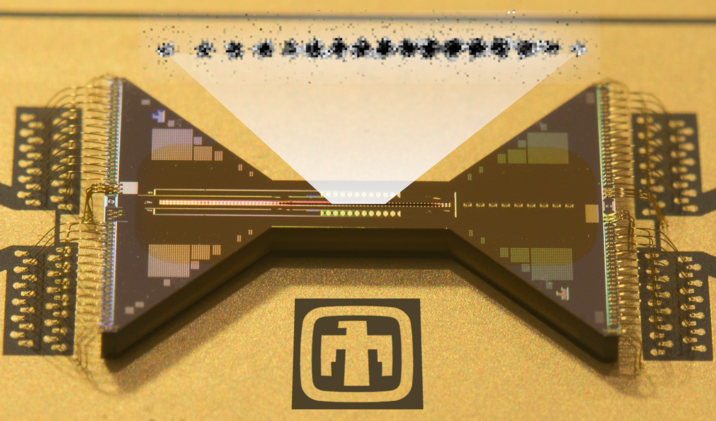
\includegraphics[width=5cm]{imgs/Phoenix_with_ion}};
      \visible<2->{
        \node at (3, -1.5) {\includegraphics[width=5cm]{imgs/Paladin_Breadboard}};
        \begin{scope}[shift={(-3, 0)}]
          \draw[line width=1] (-1.0, -3) -- node[above] {\small $|0, 0\rangle$} (1.0, -3);
          \draw[line width=1] (-1.0, -2) -- node[above] {\small $|1, 0\rangle$} (1.0, -2);
          \draw[line width=1] (-1.5, 2.5) node[left] {$^2\mathrm{P}_{1/2}$} -- (1.5, 2.5);
          \draw[line width=1,dashed] (-1.5, 3) -- (1.5, 3);
          \draw[line width=1] (-1.5, 4) node[left] {$^2\mathrm{P}_{3/2}$} -- (1.5, 4);
          \draw[blue,<->,line width=1] (-0.8, -3) -- node[left] {$355$ nm} (0, 3);
          \draw[blue,<->,line width=1] (0.8, -2) -- (0, 3);

          \draw[<->,dashed,line width=0.5] (0.95, -2) --
          node[right] {$12.6$ GHz} (0.95, -3);
          \draw[<->,dashed,line width=0.5] (1.2, 2.5) --
          node[right] {$33$ THz} (1.2, 3);
          \draw[<->,dashed,line width=0.5] (1.2, 3) --
          node[right] {$66$ THz} (1.2, 4);
        \end{scope}
      }
    \end{tikzpicture}
  \end{center}
\end{frame}

%% First generation system
% Based on these principles, our first generation EURIQA system,
% short for Error-corrected Universal Reconfigurable
% Ion-trap Quantum Archetype, is able to
% achieve high fidelity single and two-qubit operations on 15-24 qubits
% The system can not only run universally quantum circuit with high fidelity
% but is also a good platform for quantum simulation and even precision measurements.
% You can hear more about them in many other talks in this conference
% as shown in this list including one happening in a different room in an hour.

\begin{frame}{$1^{\text{st}}$ generation EURIQA system}
  \begin{center}
    \textbf{E}rror-corrected \textbf{U}niversal \textbf{R}econfigurable
    \textbf{I}on-trap \textbf{Q}uantum \textbf{A}rchetype
    \begin{columns}
      \column{5.2cm}
      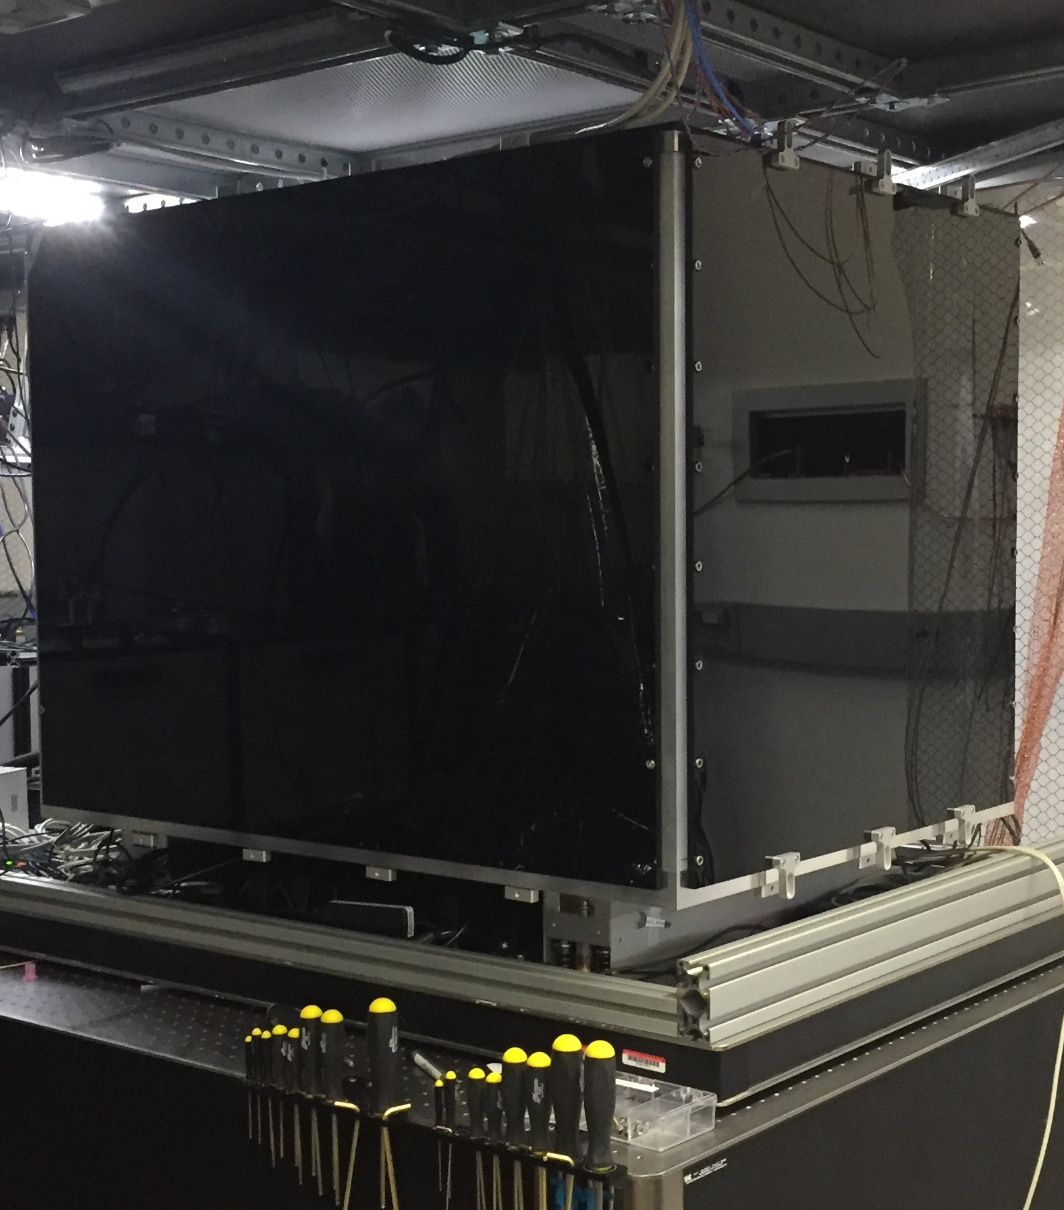
\includegraphics[width=5cm]{imgs/Breadboard_box}
      \column{6.3cm}
      \visible<2->{
        \begin{block}{}
          \begin{itemize}
          \item 15-24 usable qubits
          \item High fidelity single ($99.9\ \%$) and two-qubit ($99\ \%$) gates
          \end{itemize}
        \end{block}
        \vspace{2cm}
      }
    \end{columns}
  \end{center}
\end{frame}

%% Second generation system
% Following the success of the first system, we've designed and built
% the second generation EURIQA system to improve upon some of the limitations
% and address some of the lessons we've learnt from the first one
% with some of the new features listed here.
% The majority of the system has been assembled and I'm going to highlight some of
% these changes and focus on our initial tweak up and characterization
% of the system for the rest of the talk.

\begin{frame}{$2^{\text{nd}}$ generation EURIQA system}
  \begin{center}
    \vspace{-0.5cm}
    \begin{tikzpicture}
      \node at (0, 0) {\includegraphics[width=7.5cm]{imgs/Brassboard_render}};
      \draw[->,cyan,line width=3,>=stealth] (-3.8, 3.0) -- (-0.9, 0.5);
      \node[align=center,font=\tiny] at (-3.8, 3.0)
      {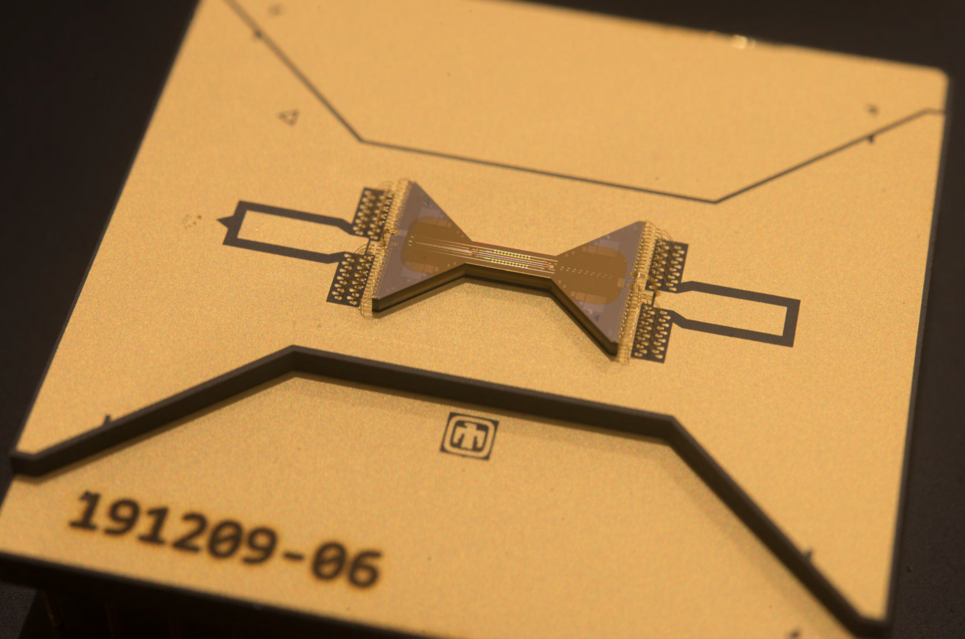
\includegraphics[width=2.3cm]{imgs/Phoenix_zoomout}\\
        Sandia Phoenix trap};
      \draw[->,cyan,line width=3,>=stealth] (-2.7, -3.0) -- (0.9, -1);
      \node[align=center,font=\tiny] at (-2.7, -3.0)
      {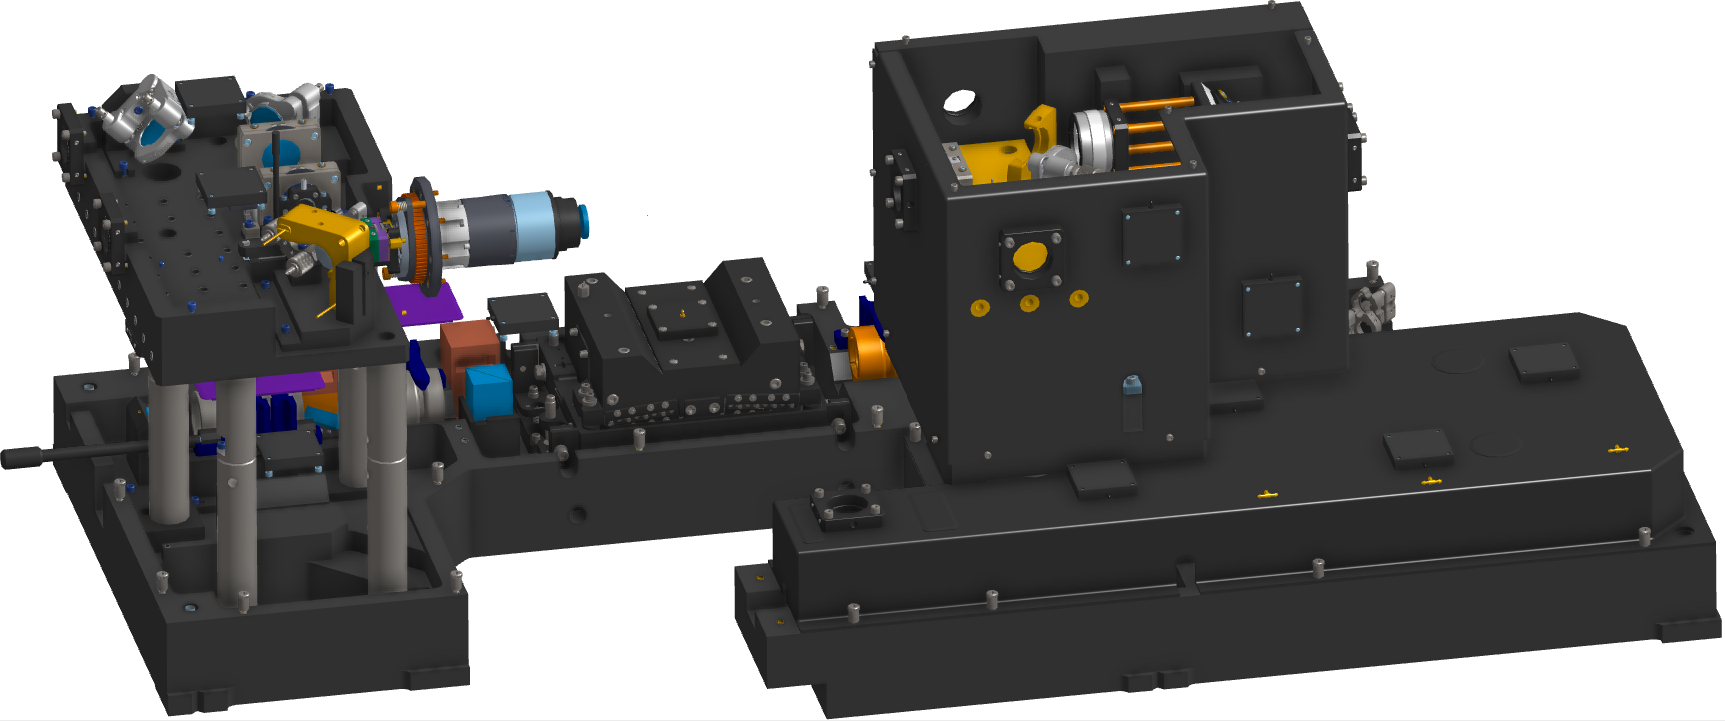
\includegraphics[width=4cm]{imgs/Harris_overview}\\
        L3Harris Raman beam path};
      \draw[->,cyan,line width=3,>=stealth] (3.9, 2.7) -- (-0.4, 1.0);
      \node[align=center,font=\tiny] at (3.9, 2.7)
      {\includegraphics[width=2.6cm]{imgs/Vacuum_stack_photo}\\
        Improved vacuum system};
    \end{tikzpicture}
  \end{center}
\end{frame}

%% Vacuum system
% One of the most basic requirement for an ion trapping experiment of course is
% the vacuum. In this generation, we used vacuum fired component that has lower
% Hydrogen content to reduce the vacuum background pressure.
% In particular, this should reduce the rate of reordering of the ion chain
% caused by collisions with background gas molecules,
% which was one of the factors limiting the usable time
% on the first generation experiment.
%
% In fact, we could measure this collision rate with the ion and infer
% our vacuum pressure. The way this works is to create a double well protential
% using our electrodes with a very weak barrier. If the barrier height
% is significantly lower than the energy imparted on the ion
% by a background collision, then every collision and the subsequent recooling
% of the ion would essentially cause the ion to settle in one of the two wells
% randomly with a 50/50 chance. The collision rate is therefore twice the rate
% the ion changes site and the rate can be converted to pressure using the known
% temperature and collision cross-section from the Hydrogen-dominated background gas.
%
% You can see the result of this measurement here on this plot.
% This is a recording of the ion position (labelled as 1 and -1)
% over just over a day. We get a site-hopping event every just under an hour.
% This corresponds to a background pressure of about 1e-11 Torr,
% which is about 5-10x better than what we got from a similar measurement
% on the first gen experiment.

\begin{frame}{$2^{\text{nd}}$ gen EURIQA: Improved vacuum}
  \begin{center}
    \begin{columns}
      \column{6.3cm}
      \begin{itemize}
      \item Vacuum fired components
      \item<2-> Reduce ion-chain reordering rate
      \item<4-> $1.32(21)\times10^{-11}\ \mathrm{Torr}$ measured pressure
      \end{itemize}
      \visible<4->{
        \begin{center}
          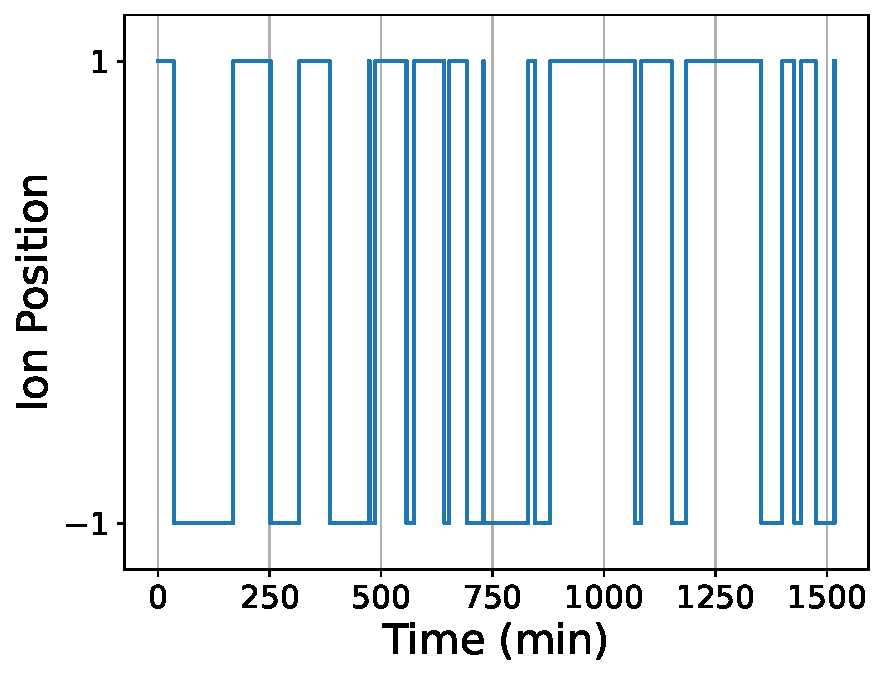
\includegraphics[width=6cm]{imgs/double-well.pdf}
        \end{center}
      }
      \column{5.1cm}
      \begin{tikzpicture}
        \node at (0, 0) {\includegraphics[width=5cm]{imgs/Vacuum_stack_photo.png}};
        \visible<3->{
          \fill[white,opacity=0.9] (-2.52, -2.63) rectangle (2.52, 2.63);
          \draw[line width=1, domain=-2.15:2.15,smooth,variable=\x]
          plot ({\x}, {0.3 * (\x)^4 - 0.7 * (\x)^2 - 1});
          \fill[red] (-1.0801234497346435, -1) circle (0.1);
          \fill[red!25!white,draw=red] (1.0801234497346435, -1) circle (0.1);

          \draw[blue,line width=1,<->,>=stealth]
          (-1, -0.9) to [bend left=40] (1, -0.9);
        }
      \end{tikzpicture}
    \end{columns}
  \end{center}
\end{frame}

%% Phoenix trap
% Another very important ingredient for an ion trap experiment is,
% well, the trap itself. In our experiment, we use a new generation of surface trap,
% called the Phoenix trap, from the Sandia national lab.
% The trap incorporated several design features that allows better and faster loading
% of the ion as well as a better electrode configuration to allow more precise
% and more flexible ion chain constrol.
%
% However, more importantly, the fabrication process of the trap is improved
% to reduce the electric field noise caused by the trap surface.
% Such noise could cause heating of the ion motion and this,
% especially the heating on the axial motional mode of the ion,
% was one of the main limiting factor on the two qubit gate fidelity
% on the first generation system.
%
% We measured the heating rate of the ion by holding the ion in the dark
% for a variable length of time and then measure it's temperature
% by driving a motion sensitive transition on the 435 nm line
% to the metastable D state. The measured heating rate is plotted here as a function
% of the trapping frequency. These numbers are consistent with the measurements
% by Sandia and we can also compare it to what we measured on the first gen system
% as shown by this green point here. Our heating rate appears to be about 3x better
% than the first gen number which should give us an improvement in the 2 qubit gate
% fidelity because of this, especially for long circuits.
% We are very grateful that Sandia could make such a major improvement
% in the trap design.

\definecolor{trapyellow}{HTML}{ffe0a5}
\definecolor{semgray}{HTML}{cccccc}

\begin{frame}{$2^{\text{nd}}$ gen EURIQA: Phoenix trap}
  \begin{center}
    \begin{tikzpicture}
      \node at (3, 2) {\includegraphics[width=4.8cm]{imgs/Phoenix}};
      \visible<2-3>{
        \fill[semgray,opacity=0.6] (1.8, 2.115) -- (-4.65, -0.3875)
        -- (-0.35, -3.6125) -- (1.9, 2.115) -- cycle;
      }
      \visible<4>{
        \fill[semgray,opacity=0.2] (1.8, 2.115) -- (-4.65, -0.3875)
        -- (-0.35, -3.6125) -- (1.9, 2.115) -- cycle;
      }
      \node[text width=6.5cm] at (-3, 2) {
        \begin{itemize}
        \item<2-> Better loading and chain control
        \item<3-> Reduced surface electrical noise\\
          \uncover<-2,4->{3x less heating compared to EURIQA-1}
        \end{itemize}
      };
      \visible<2-3>{
        \fill[trapyellow,opacity=0.6]
        (2.85, 2.115) -- (0.9, -1) -- (5.7, -1)
        -- (3.15, 2.115) -- cycle;
        \node at (3.3, -2) {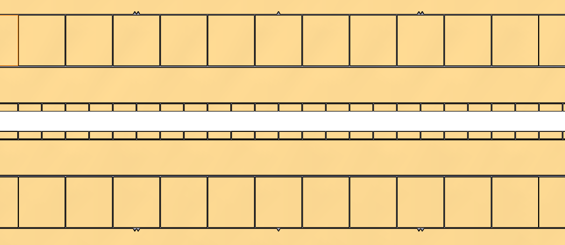
\includegraphics[width=4.8cm]{imgs/Phoenix_quantum}};
        \node at (-2.5, -2) {\includegraphics[width=4.3cm]{imgs/Phoenix_Loading_SEM}};
      }
      \visible<4>{
        \fill[trapyellow,opacity=0.15]
        (2.85, 2.115) -- (0.9, -1) -- (5.7, -1)
        -- (3.15, 2.115) -- cycle;
        \node[opacity=0.25] at (3.3, -2) {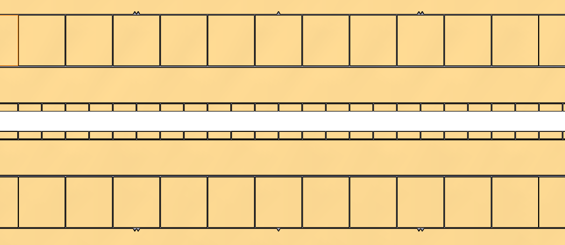
\includegraphics[width=4.8cm]{imgs/Phoenix_quantum}};
        \node[opacity=0.25] at (-2.5, -2) {\includegraphics[width=4.3cm]{imgs/Phoenix_Loading_SEM}};
        \node at (-0.5, -1.8) {\includegraphics[width=7cm]{imgs/heating-rate}};
      }
      \node[align=left,font=\tiny] at (3.8, -4.3)
      {F01.00038 The Quantum Scientific Computing\\
        \phantom{F01.00038} Open User Testbed (QSCOUT)};
    \end{tikzpicture}
  \end{center}
\end{frame}

\begin{frame}{$2^{\text{nd}}$ gen EURIQA: New Yb atom source}
  \begin{center}
    \begin{columns}
      \column{6cm}
      \begin{itemize}
      \item Sympathetic cooling with $^{172}\mathrm{Yb}^+$\\
        {\scriptsize Cetina, et al., PRX Quantum 3, 010334 (2022)}\\
        \vspace{1em}
      \item<2-> New Yb source to enhance loading of $^{172}\mathrm{Yb}^+$
      \end{itemize}
      \vspace{1em}
      \visible<2->{
        \begin{center}
          \includegraphics[width=4.5cm]{imgs/Loading_Frequency.png}
        \end{center}
      }
      \column{5.5cm}
      \includegraphics[width=5.5cm]{imgs/AxialCooling.pdf}
      \vspace{2cm}
    \end{columns}
  \end{center}
\end{frame}

% T2
% With the ion trapped and cooled, we can now take care of the qubit aspect of the ion.
% As previously mentioned, the coherence time for the mF=0 hyperfine qubit is generally
% very good due to it's natural low sensitivity to magnetic field fluctuation.
% We measured this in our experiment using a standard microwave Ramsey experiment
% with spin-echo and the sequence is shown here.
% The decay of the oscillation contrast is plotted here as a function of the wait time.
% which give us a coherence time of 2.7 seconds, not quite the world record but
% plenty long enough for most of our circuits.
% We believe this is currently limited by the residue sensitivity to B field noise
% and it should further improve once we've implemented
% the planned magnetic field shielding.

\begin{frame}{$2^{\text{nd}}$ gen EURIQA: Qubit coherence}
  \begin{center}
    \begin{tikzpicture}
      \draw[orange,fill=orange!50!white,line width=1] (0.45, 3.5) rectangle (0.75, 4.5);
      \node[above] at (0.6, 4.5) {\scriptsize $R_x(\pi/2)$};

      \draw[red,fill=red!50!white,line width=1] (2.7, 3.5) rectangle (3.3, 4.5);
      \node[above] at (3, 4.5) {\scriptsize $R_x(\pi)$};

      \draw[orange,fill=orange!50!white,line width=1] (5.25, 3.5) rectangle (5.55, 4.5);
      \node[above] at (5.4, 4.5) {\scriptsize $R_\varphi(\pi/2)$};

      \draw[->,>=stealth,line width=1] (0, 3.5) -- (6, 3.5);

      \draw[line width=0.7] (0.6, 3.5) -- (0.6, 3.1);
      \draw[->,>=stealth,line width=1] (2.5, 3.3) -- (0.6, 3.3);
      \draw[line width=0.7] (5.4, 3.5) -- (5.4, 3.1);
      \draw[->,>=stealth,line width=1] (3.5, 3.3) -- (5.4, 3.3);
      \node at (3, 3.3) {$t$};

      \visible<2->{
        \node at (2.65, 0) {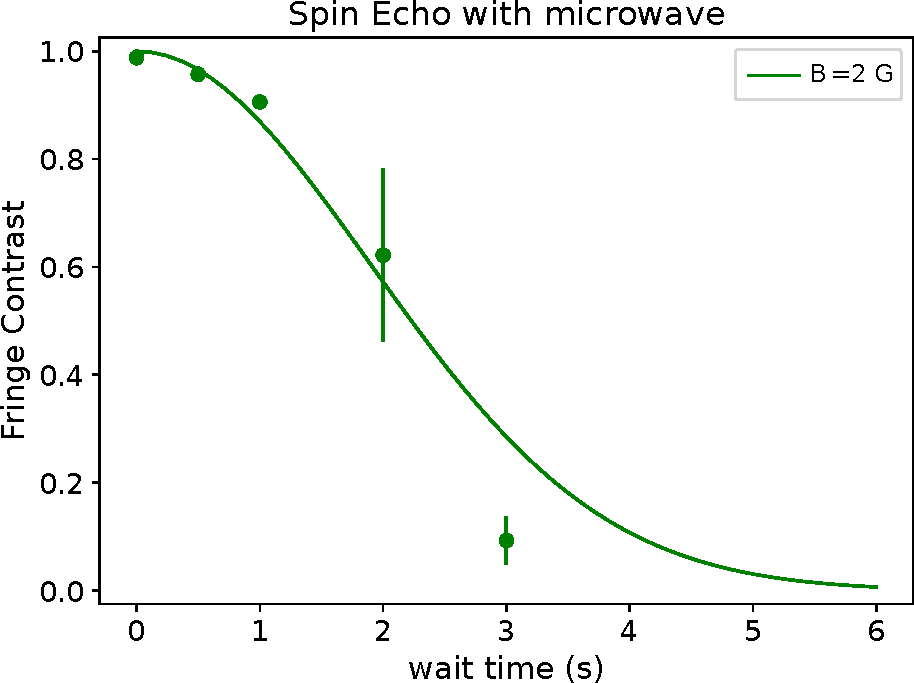
\includegraphics[width=6.8cm]{imgs/t2}};
      }
      \node[text width=5cm] at (-3, 3) {
        \begin{itemize}
        \item<1-> Ramsey with spin-echo\\
          using microwave
        \item<2-> $T_2=2.68(36)\ \mathrm{s}$\\
          {\scriptsize (Can be further improved with shielding)}
        \end{itemize}
      };
    \end{tikzpicture}
  \end{center}
\end{frame}

% Imaging
% Just like our first system, the universality is achieved via individual addressing
% and detection of the ion internal state. Here we use
% the same high numerical aperture objective to collect the photons from the ions.
% The light is then focused onto an array of multi-mode fibers through a second
% imaging stage to allow us to distinguish between the signal from different ions.
%
% This system was aligned and here you can see the signal we got on different
% photo-multiplier tubes as we move a single ion across the trap axis.
% The detection extinction is very good and we measured
% a nearest neighbor cross-talk of about 0.05%.
\begin{frame}{$2^{\text{nd}}$ gen EURIQA: Imaging system}
  \begin{center}
    \begin{tikzpicture}
      \node at (-3.2, 2) {\includegraphics[width=4.5cm]{imgs/photon-gear}};
      \visible<2->{
        \node at (-3, -2.2) {\includegraphics[width=6cm]{imgs/imaging_combined.pdf}};
      }
      \visible<3->{
        \fill[gray,opacity=0.4] (-5.75, -1.22) -- (-0.25, -1.22) -- (-4.74, -2.2) -- (-5.545, -2.2) -- cycle;
        \node at (-3, -1.1) {\includegraphics[width=5.5cm]{imgs/fiber_bundle_tip_zoomin.png}};
      }
      \visible<4->{
        \node at (2.8, -0.2) {\includegraphics[width=6cm]{imgs/pmt-array.png}};
      }
      \node[text width=5.7cm] at (3, 3.6) {
        \begin{itemize}
        \item<1-> NA=0.63 lens.
        \item<2-> 32 channel fiber bundle for individual detection.
        \item<4-> Crosstalk between neighboring channels: $0.05 \%$
        \end{itemize}
      };
    \end{tikzpicture}
  \end{center}
\end{frame}

% Raman
% With the coherence of the ion motion and internal state under control
% and with the ability to detect the state of individual ions,
% the final main ingredient for our quantum computer is the quantum gate,
% which, as I mentioned earlier, is realized using Raman transitions
% coupling the two qubit states.
% We use a counter-propagating Raman beam geomety parallel to the trap surface.
% This offers us a weaker sensitivity to surface noise heating
% and also potentially faster gate speed due to a larger momentum kick
% compare to the previous generation. Just like the first generation,
% we have a single global beam on one side shared by all the ions
% and 32 individual beams on the other side for, well,
% individual addressing of each individual ions.
% We have aligned both of the beams onto the ions and you can see here is a nice
% carrier spectrum driven by both the global and individual beams.
% Just like for the individual detection, it's important that each of the individual
% beams only addresses their corresponding ions. We can use a very similar method
% to measure this as well by moving the ion and observe their response to different
% individual beams. As you can see in this plot, the signals from different beams
% are fairly well separated and we've measured a crosstalk between neighbor ions
% at about 2% and between further ions to be almost negligible.
% We expect the final fine alignment of the beam could improve this
% a little bit and we'll implement crosstalk cancellation
% which was shown in the previous system to be able to cut this down by another 10x.

\begin{frame}{$2^{\text{nd}}$ gen EURIQA: Raman addressing}
  \begin{center}
    \begin{tikzpicture}
      \node at (0, 0) {\includegraphics[width=8cm]{imgs/Brassboard_Raman.png}};

      \node[rotate=90] at (4.5, 0) {
\includegraphics[width=7cm]{imgs/Global_beam.png}};
      \node[rotate=90] at (-4.5, 0) {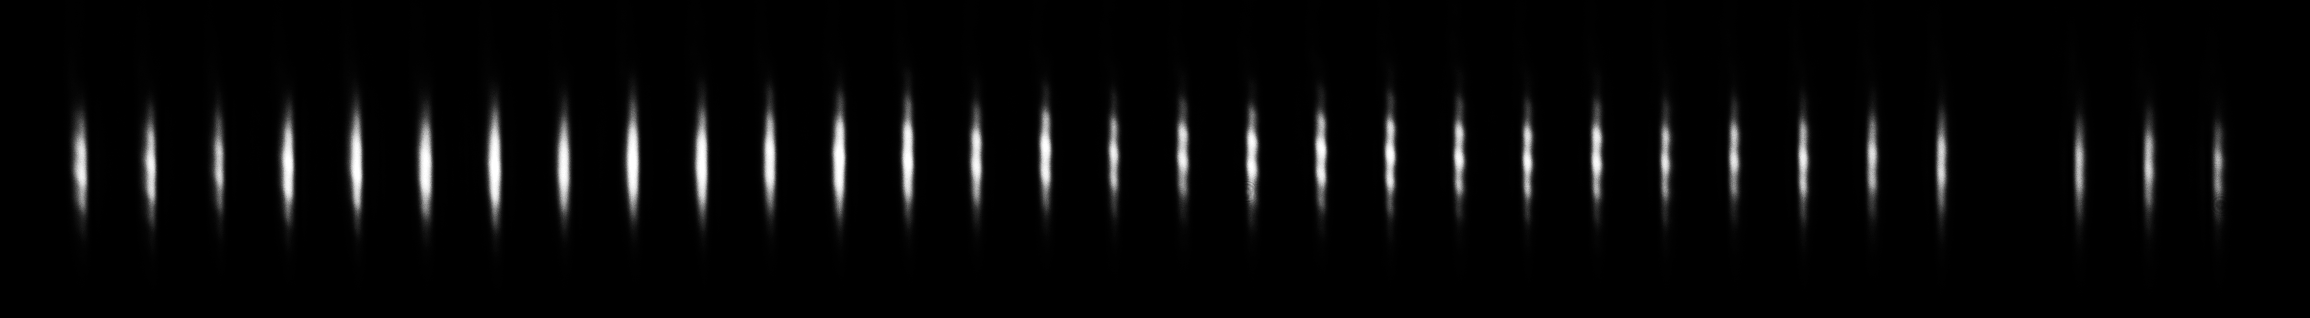
\includegraphics[width=5.4cm]{imgs/Individual_beam.png}};
      \visible<2->{
        \fill[white,opacity=0.9] (-4.9, -3.6) rectangle (4.9, 3.6);
      }
      \visible<2->{
        \fill[white,path fading = north edge fading] (-5.75, -3.2) rectangle (-.34, 2);
      }
      \visible<3->{
        \fill[white,path fading = north edge fading]
        (5.75, -3.62) rectangle (.32, 2);
      }

      \node[text width=8cm] at (0, 3) {
        \begin{itemize}
        \item<1-> Counter-prop global and individual beams
        \item<2-> Cross-beam Raman signal
        \item<3-> Individual addressing\\
          Nearest neighbor crosstalk: $2\%$.
        \end{itemize}
      };
      \visible<2->{
        \node at (-3, -1) {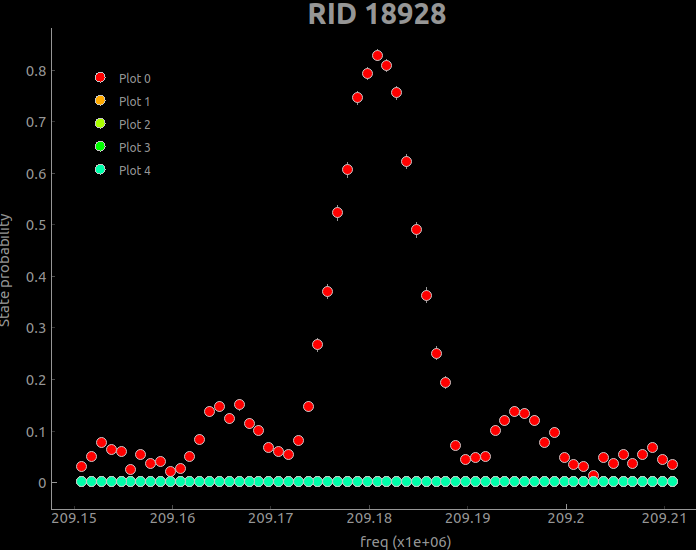
\includegraphics[width=5.5cm]{imgs/Raman_spectrum}};
      }
      \visible<3->{
        \node at (3, -1) {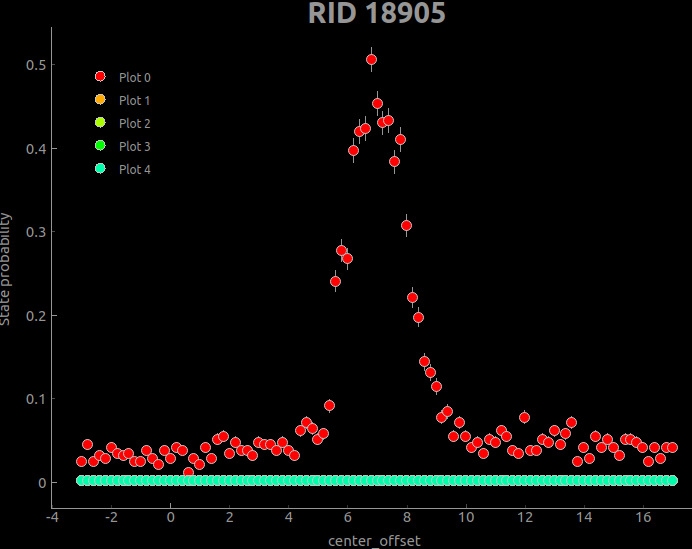
\includegraphics[width=5.5cm]{imgs/Raman_profile}};
      }
    \end{tikzpicture}
  \end{center}
\end{frame}

% TODO: MS gate

% With that
{
  \usebackgroundtemplate{
    \makebox[\paperwidth][c]{\centering\includegraphics[width=\paperwidth]{imgs/LabPicture_bg.png}}
  }
  \begin{frame}{}
    \begin{center}
      \begin{tikzpicture}
        \shadedraw[inner color=gray,outer color=blue!40!white,path fading = glow2 fading] (-5.8,0.05) rectangle (1.8,0.15);
        \shadedraw[inner color=gray,outer color=blue!40!white,path fading = glow2 fading] (2.2,0.05) rectangle (5.8,0.15);

        \node[align=center,below,font=\tiny] at (-5, 0)
        {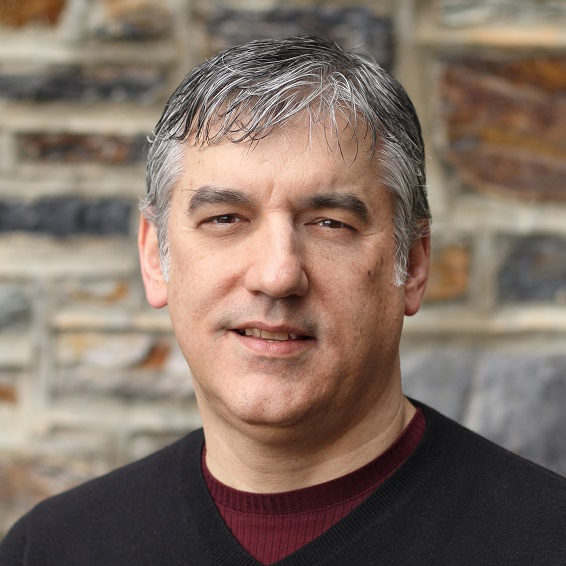
\includegraphics[height=1.7cm]{imgs/members/Chris.jpg}\\Christopher R Monroe};
        \node[align=center,below,font=\tiny] at (-3, 0)
        {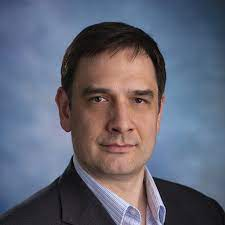
\includegraphics[height=1.7cm]{imgs/members/Alex.jpg}\\Alexander Kozhanov};
        \node[align=center,below,font=\tiny] at (-1, 0)
        {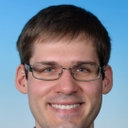
\includegraphics[height=1.7cm]{imgs/members/Marko.jpg}\\Marko Cetina};
        \node[align=center,below,font=\tiny] at (1, 0)
        {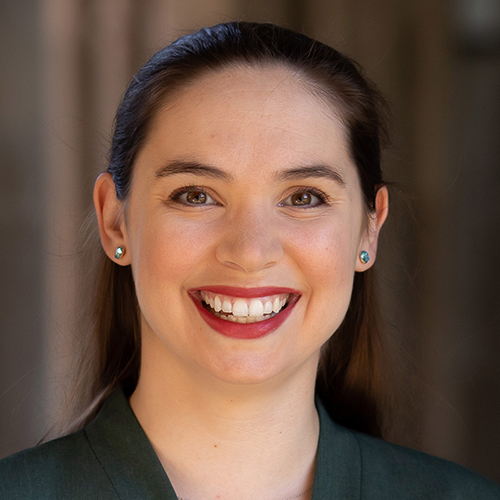
\includegraphics[height=1.7cm]{imgs/members/Crystal.jpg}\\Crystal Noel};
        \node[align=center,below,font=\tiny] at (3, 0)
        {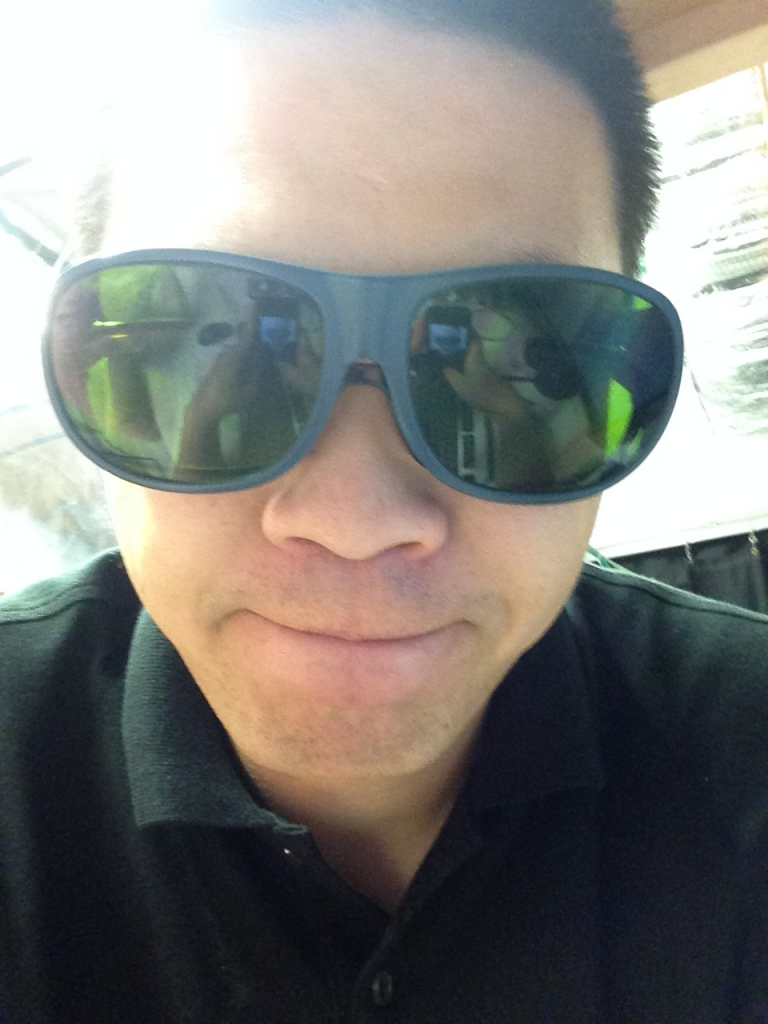
\includegraphics[height=1.7cm]{imgs/members/Lei.png}\\Lei Feng};
        \node[align=center,below,font=\tiny] at (5, 0)
        {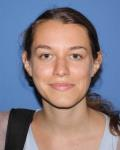
\includegraphics[height=1.7cm]{imgs/members/Mila.jpg}\\Liudmila Zhukas};

        \shadedraw[inner color=gray,outer color=blue!40!white,path fading = glow2 fading] (-5.8,0.05-3) rectangle (5.8,0.15-3);

        \node[align=center,below,font=\tiny] at (-5, -3)
        {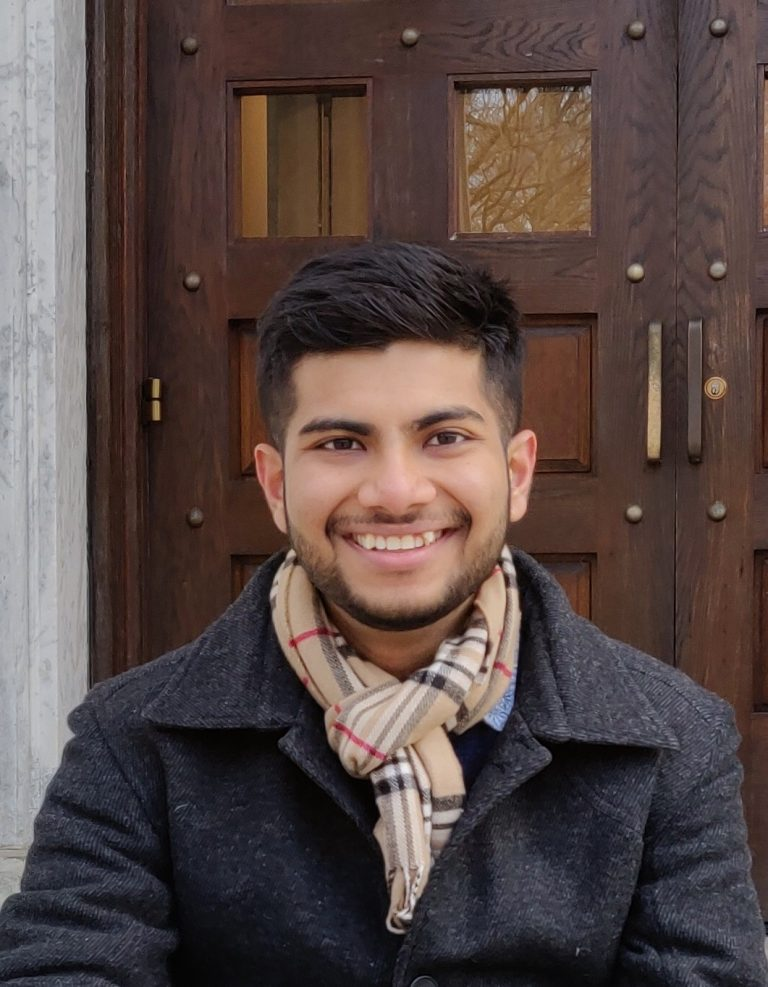
\includegraphics[height=1.7cm]{imgs/members/Debo.jpg}\\Debopriyo Biswas};
        \node[align=center,below,font=\tiny] at (-3, -3)
        {\includegraphics[height=1.7cm]{imgs/members/Vivian.png}\\Vivian Zhang};
        \node[align=center,below,font=\tiny] at (-1, -3)
        {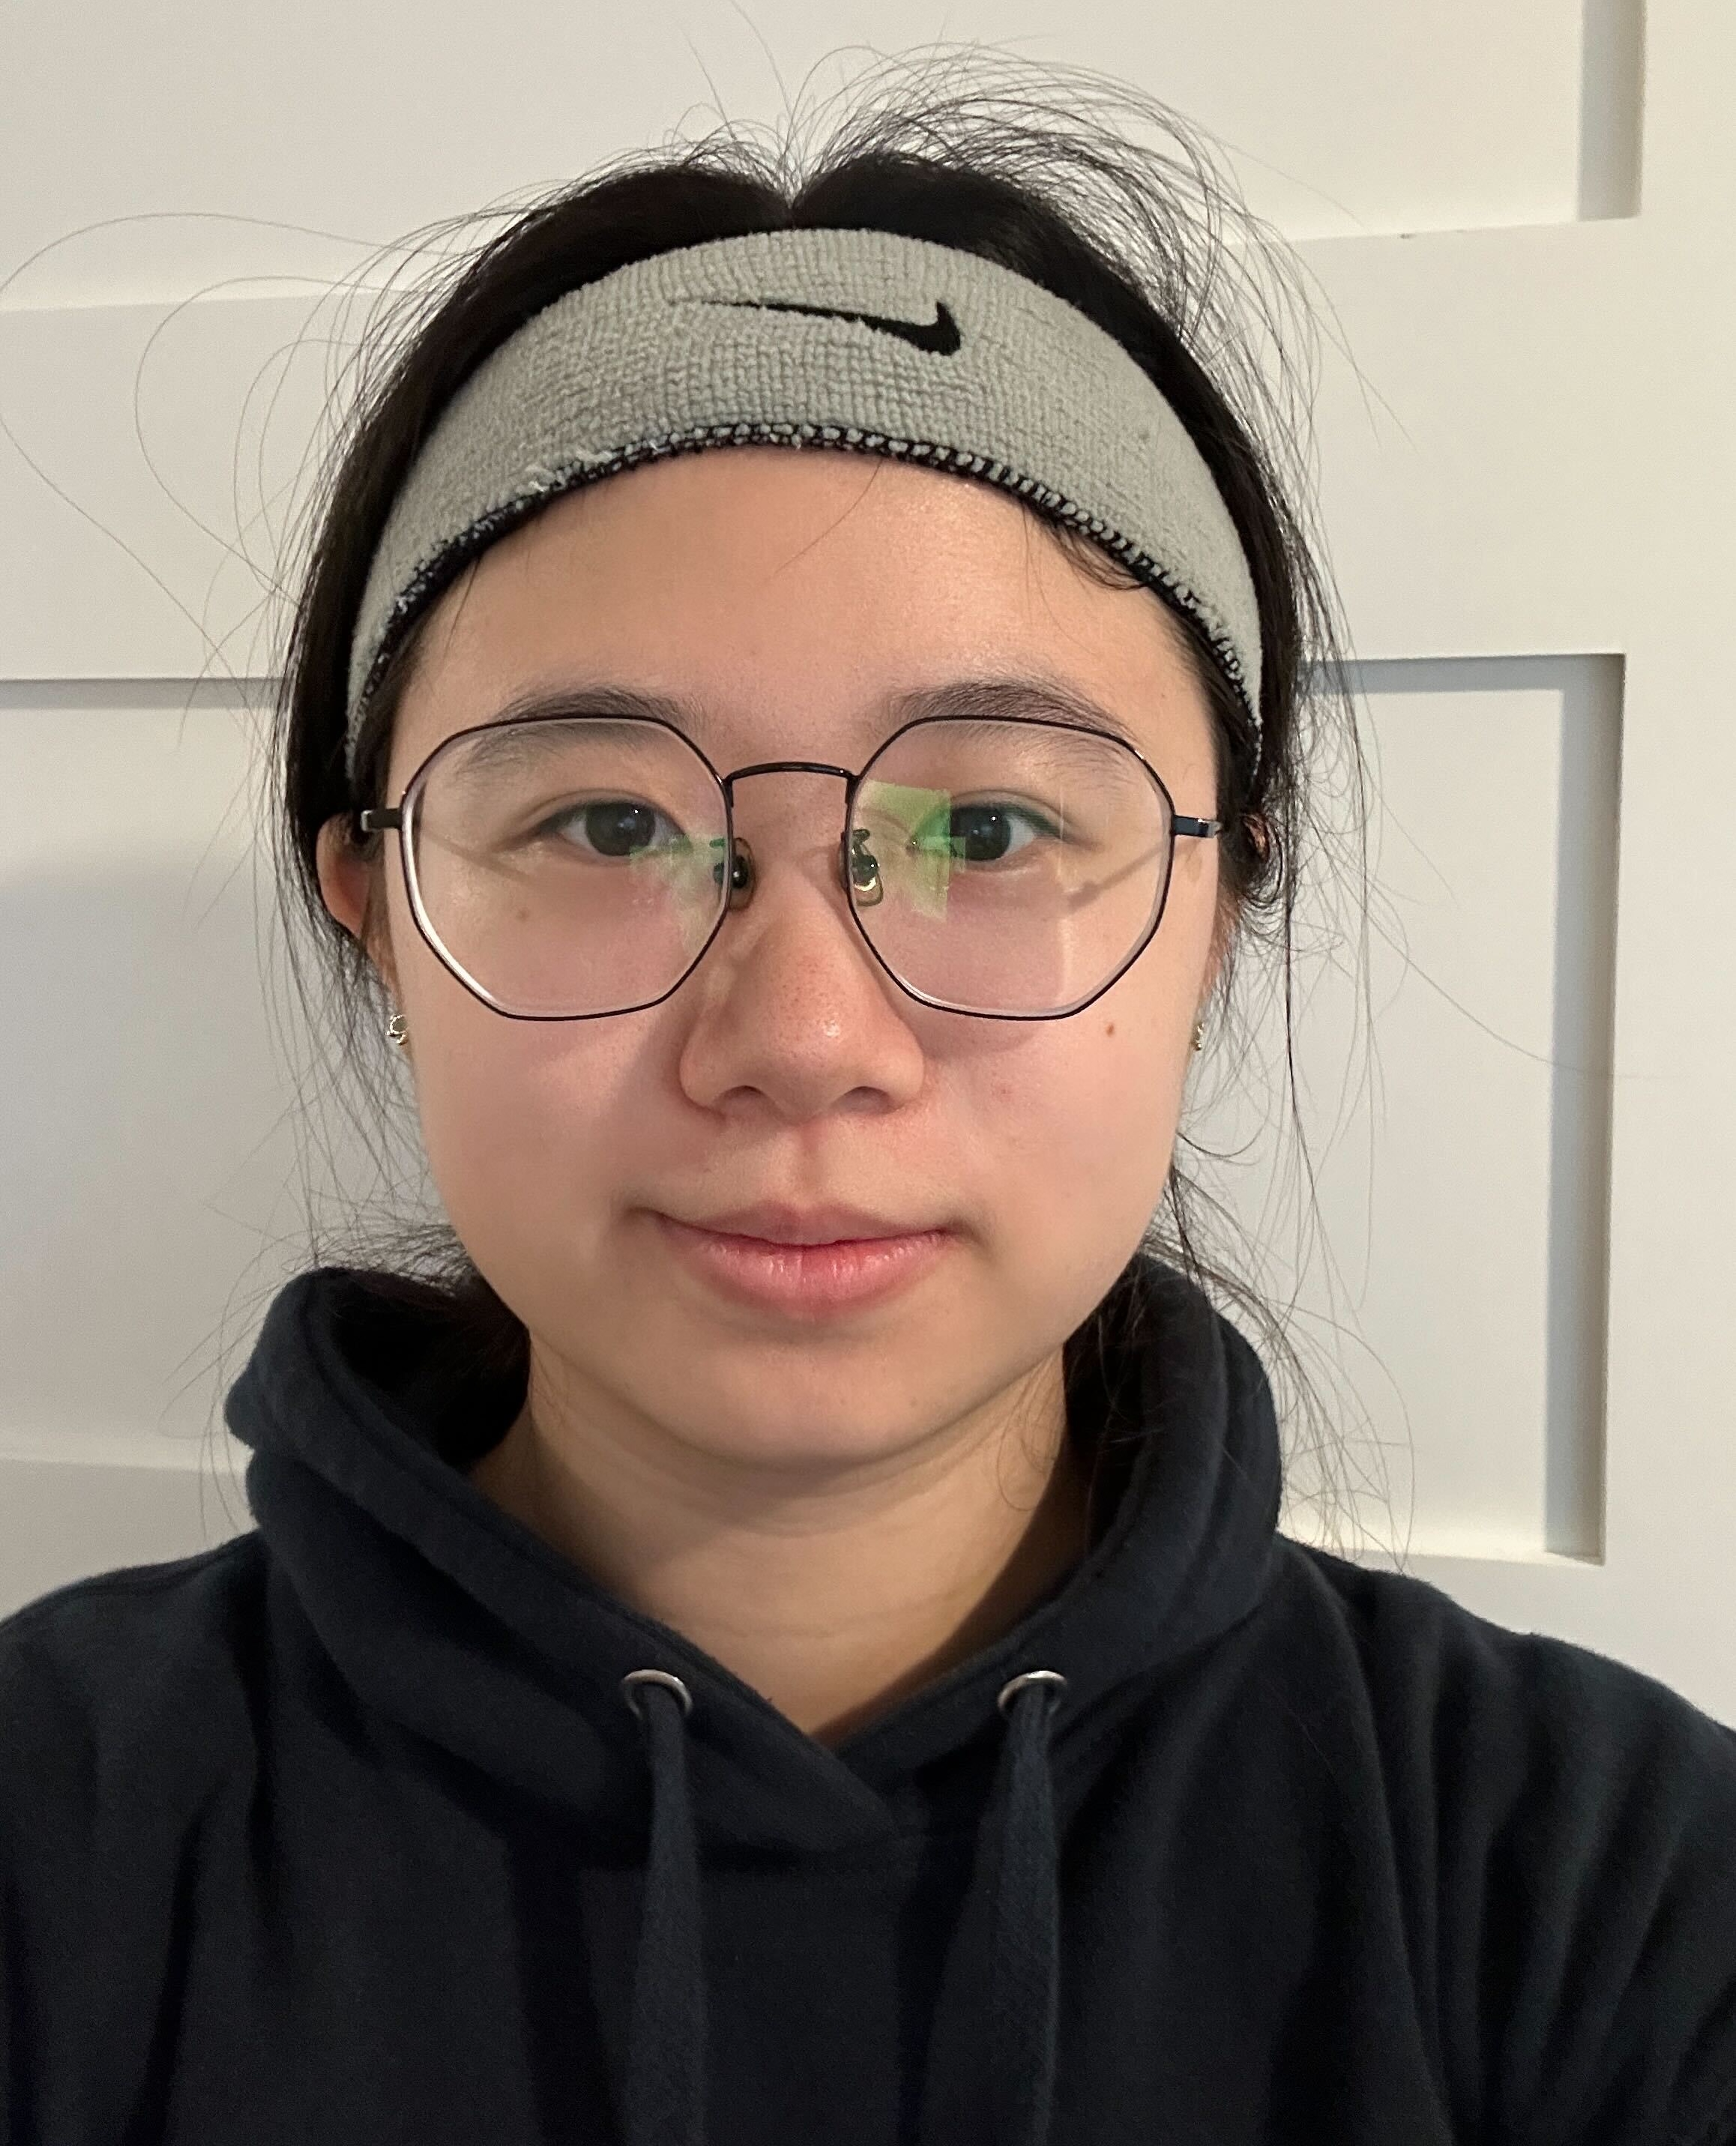
\includegraphics[height=1.7cm]{imgs/members/Keqin.jpg}\\Keqin Yan};
        \node[align=center,below,font=\tiny] at (1, -3)
        {\includegraphics[height=1.7cm]{imgs/members/Bahaa.jpg}\\Bahaa Harraz};
        \node[align=center,below,font=\tiny] at (3, -3)
        {\includegraphics[height=1.7cm]{imgs/members/Grant.jpg}\\Grant Eberle};
        \node[align=center,below,font=\tiny] at (5, -3)
        {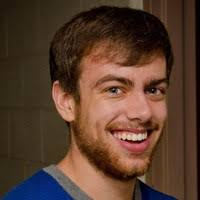
\includegraphics[height=1.7cm]{imgs/members/Drew.jpg}\\Andrew Risinger};
      \end{tikzpicture}
    \end{center}
  \end{frame}
}

\begin{frame}{}
\end{frame}

\end{document}
